\documentclass[]{article}
\usepackage[pdftex]{graphicx}
\usepackage[top=1in, bottom=1in, right=1.25in, left=1.25in]{geometry}
\usepackage{hyperref}
\hypersetup{colorlinks=true, linkcolor=blue, urlcolor=blue}

\begin{document}
	\pagenumbering{roman}
	\tableofcontents
	\newpage
	\pagenumbering{arabic}
	\setcounter{page}{1}
	\thispagestyle{empty}
	
	
	% Twelfth Entry
	\section{Scheduling for Remainder of Semester}
		With Colin and Griffin
	
	
	% Eleventh Entry
	\section{Adding Meeting Minutes and Additional Features 10/12/2012}
		
		\subsection{Re-format Site}
			When adding the minutes to the website, the file browser started to look cluttered so the layout of the site was changed to be a list where each entry represents a meeting. Each meeting has a name, a minutes file, an agenda file, and the date the meeting occurred on. This system appears to organize the site as well as allows for storage of files on github via a hyperlink. The reasoning behind this is to not use up the quota on the Google site, which is limited. By making an open project on github, the project is guaranteed unlimited space. 
			
		\subsection{Finishing Touches on Tech Specs}
			After reviewing the feedback from meetings, I realized that I needed to add a comment about how resolution will not be a problem for the project since the Microsoft paper used a 4MP camera 10 years ago and it was not a problem.
		
	% Tenth Entry
	\section{Finishing Technical Specifications 10/11/2012}
		To make sure that the work done in this worklog appears on time on the ProPANE website, I have removed the file from the site and replaced it with the link to the worklog on github. This will insure that on every push the worklog gets updated on the site. Have successfully tested this method and it works.\\
		
		\subsection{Note on Git Usage}
			Forgot to pull down before editing and git gave a message like:\\
			\includegraphics[scale=0.5]{images/git-problem1.jpeg}\\
			To fix this, I added the top and bottom tex files listed in the modified list. Committing again resulted in an error free commit.\\
			Need to remember to pull before editing. 
			
		\subsection{Addition of Priorities}
			Prioritized the technical specifications based on the following qualifications. The priority is HIGH if a violation of the specification would result in a non-functional system. The priority is MEDIUM if a violation of the specification would result in a functional, but non-usable system. The priority is LOW if a violation of the specification would result in a functional usable, but difficult to use system. \\
			\\
			A HIGH priority spec is essentially a 'mission critical' specification. Violation of a MEDIUM priority spec essentially says that the system is capturing and analyzing the images, but it is violating the portability requirement for the system. Violation of a LOW priority spec basically says that the system is functional and portable, but will require extra resources (time, software, etc) to use.
			
	% Ninth Entry
	\section{Group Meeting for PSM 1 10/01/2012}
		The main issues discussed were the resolution issue and the interface issue that were brought up during the initial panel. The resolution issue was basically the agreement with the clients that there will have to be a certain number of pixels given to a certain portion of the board. The interface issue is that not all professors would feel comfortable using Linux for the analysis system. 
		
		\subsection{Resolution Issue}
			This does not seem like it will be an issue because the Microsoft paper shows that the goals we wish to accomplish were accomplished using a 4 MP camera from 10 years ago. Given that the setup for data collection in the paper is nearly the same as what we are using, the progression in camera technology should not be a problem.\\
			\\
			However, this IS an issue because it is an area that could possibly pose legal problems. If the resolution is too poor, then the system would be giving ProPANE reliant students a disadvantage. In my opinion, that would be a complete failure of the project.
			
		\subsection{Interface Issue}
			This issue could pose a problem for the project and will have to be investigated. Given that professors do not want to interact with any of the Linux GUIs (and there is no reason why they should). We will have to find a way to browse/export (key) images through a classic interface (i.e. OS X, Windows 7, Windows Vista). The three options I see for solving this problem are: creating our own GUI, give path names, or make a separate directory. 
			
			\subsubsection{ProPANE GUI}
				Creating a GUI would be an extra step in the project and it seems like it would fall under the category of scope creep (let's save this for version 2, but make initial notes on what it will have to do).\\
				\\
				The GUI would have to be cross platform and not require anything special (make it accessible to everyone). To me this sounds like a website. Given my website skills (PHP, Ruby on Rails, MySQL, AJAX etc), this seems like the best way to go. Everyone is comfortable using a browser so it would relatively simple to create the GUI.
				
			\subsubsection{Path Names}
				Theoretically the analysis system would generate key images and know the path to the key images. If everything is kept in an SMB share (where security will already be taken care of), users would be presented clickable links to the key images that would be on the share. This would require an image browser/editor on the client computer, but relatively little work for the group.
				
			\subsubsection{Separate Directory}
				Basically, this would have the analysis system have a directory titled ``All\_Images" and one titled ``Key\_Images". This would make life incredibly easy because a key image would just have to be copied from all images to key images. However, the drawback is that since the key images will not be living near images taken at around the same time. If the key image is wrong, the professor would have to go back to all images and search for the key image and then find the the correct key image. The above system would allow for this with just an arrow key action. 
	
	% Eigth Entry
	\section{Review of Panel 1 Notes 09/28/2012}
		
		\subsection{Tech Specs}
			Judging by the reactions of the panel members, the technical specifications are coming along well. The idea of the analysis system being run on a Linux platform brought up a problem that some professors will not be comfortable using Linux and would prefer OS X or Windows. It seems like a good idea to keep the actual analysis on Linux (keep it open!), but there will have to be an easy to access interface for browsing images. The first thing that came to mind was a web interface. A web interface would be a good idea because it is platform independent and it makes GUI programming a lot easier than using something like QT. It might also allow for integration with Moodle. \\
			\\
			By removing the capture environment entirely, the project has become too loose with environment requirements. I need to determine the coarsest requirements that the system will have to meet. Basically, the system has to operate somewhere between 3 feet away from the board and the back of a classroom. This does not limit the design, it just insures that it will be practical. 
			
		\subsection{Future Trade Analysis}
			Professor Thompson brought up that there are more than just the Samsung Android powered cameras. For example, there is a Nikon one \href{http://www.engadget.com/2012/08/22/nikon-coolpix-s800c-android-camera-pricing-ship-date-details/}{here}.\\
			\\
			The trade analysis will require finding as many of these products as possible and ranking them based on the requirements that the team comes up with. This means that in addition to the research, we need to sit down as a group and hash out what the camera requirements will be. 
	
	% Seventh Entry
	\section{Finializing Tech Spces for First Panel 09/25/2012}
		
		\subsection{Meeting with Thompson}
			The big change that has to be made is to enumerate the steps for using the ProPANE system. This will be crucial for the members of the panel to understand what we want the system to do. Also, the technical specifications document needs to be trimmed down so that it only contains the basic constraints imposed by Dr. Midkiff and Dr. Gabauer. 
			
		\subsection{Generating Sequence for Use}
			The basic outline for a professor to use is: setup the capture system in a classroom, start the capture system, use the board, stop the capture system, browse analysis system for desired frames, and finally export images to where they are needed. This sequence will take the user from having nothing to having all of the images captured during the lecture, which are ready to be sent to students. 
			
		\subsection{Pruning Tech Specs}
			The goal of pruning the tech specs is to give the group as few restrictions as possible to get the project done. Obviously, we want to deliver the best possible product, but it is still a version 1 product so giving it numerous specific requirements that are not relevant to the core needs is not helpful for development. I removed the capture environment section because it is something that will mostly be determined by the capture device. We will have to determine the limits of the capture environment at the conclusion of the project and publish them in the user manual, but right now they cannot constrain the system. 
			
			\subsubsection{Capture Environment Removals}
				Visual capture field, distance from board, viewing angle, lighting
				
			\subsubsection{Distractions Removals}
				Visual profile, audio output, visual distractions
				
		\subsection{Further Refinement}
			The idea of portability needs to be defined in a more concise fashion. Right now, the height and weight are the quantitative measures of portability, but it seems like there are ways that a portable system would violate these constraints and that an unportable system would conform to these constraints. 
				
	
	% Sixth Entry
	\section{Preparing Tech Specs for potential meeting on 9/24 09/21/2012}
		Scheduling a meeting with Prof Thompson for Monday to discuss technical specifications. Making changes to the technical specifications based on preliminary feedback. Continuing work from last night on overview and scope.
		
		\subsection{Additional Research}
			During class meeting, did some preliminary research into products that could be suitable for the capture device. Established some requirements for the capture deice. The capture device must be programmable to the extent that it can be set to take a pictures at a regular interval. The capture device must be able to transmit the pictures wirelessly. Finally, it would be nice if the capture device were completely self contained. Basically, I don't want to use a camera that is connected via USB to a computer because that would take a long time to set up and would go against the goal of portability. \\
			\\
			There are several types of technologies that I came across. The first was \href{http://www.eye.fi/}{Eye-Fi} which is an SD card that has Wifi capabilities. It would have to be used with a programmable camera and I don't know how to specify where the uploaded images go. The second technology was the iPod Touch or similar devices. The appeal for these devices is that they have cameras and connectivity that was designed to be programmable. The downside of these is that they are expensive and the camera may not be very good. The third technology is the Samsung GALAXY Camera which appears to be a camera that runs Android. It would be perfect for what this project needs because it is has the necessary camera abilities as well as the programmable interface for the connectivity. 
			
		\subsection{Tech Spec Feedback Questions}
			For the system performance feedback comment, the decision making does not have to be \%100 does it? The data gathering does have to be \%100 and because all of this there is no reason that the decision has to be \%100. The purpose of the decision making is to ease the life of the professor. \\
			\\
			As for the capture environment, should it be based on the capture device or the setup in the classrooms? 
			
		\subsection{Collectiong Testing Numbers}
			Need to collect data about capture environment. Have to measure the distance between the front desk in a classroom and the board in numerous different rooms to get a minimum and maximum distance from the board. The viewing angle and capture field will be based off of the size of a whiteboard and the minimum/maximum distance from the whiteboard to where the capture system will be located in the room. The lighting will have to be based off of the illumination level in a classroom with the lights on. \\
			\\
			If the distractions section of the tech specs document is to be kept, they need to be defined using numbers. For the visual distraction section, we will need to take pictures of a student from one desk behind to determine the actual numbers for taking up visual space. For collecting the audio data, we will have to record a projector running in an otherwise silent room to determine the maximum volume spikes and the ambient noise level.
			
	
	% Fifth Entry
	\section{Individual Work on Technical Specifications Document 09/20/2012}
		Beginning work on overview and scope. Wording is hard to get right for the analysis system. Need to define the distinct parts of the system before the use cases. Sequence of steps for use cases need to stay general or they end up specifying implementation details. 
		
			\subsection{Add to To-Do List}
				Perform research and trade analysis on image capturing systems to determine the optimal choice for the capture device.\\
				Set up meeting with Professor Thompson to iron out more details on the technical specifications.
				
			\subsection{Notes}
				The technical documents require a lot more time than they appear initially. The PDFs on Moodle provide a great way to get started on the documents. The technical specifications document needs to be completed before the implementation phase. Otherwise, the project could lose focus (scope creep). The research deliverable might have to be updated if new technologies come over the course of the next month.
	
	% Fourth Entry
	\section{Individual Work on Technical Specification Document 09/12/2012}
		Beginning to complete the sections laid out on 09/11/2012. Difficult to find the right phrasing that is precise, concise, and unambiguous. Trying to use measurements that an electronic device makes instead of a human. \\
		
		\subsection{Overview and Scope}
			This section of the document is directed at describing the overall solution. The is no solution at this point. At the moment, I have broken down the overall system into components that do not lock the team into a specific implementation, but allows for the generation of technical specifications. The breakdown of the solution is as follows: the ProPANE system is composed of a \emph{capture system} and \emph{analysis system}. The capture system is responsible for collecting all of the information presented in a class. The analysis system will be the part that does all the image processing, display of images, selection of key frames, exportation features, and anything else that does not collect data. The capture system can then be broken down into a capture device and a communication device. The capture device gathers the information presented in a class and the communication device sends the data to the analysis system. These different components do not have to map to different pieces of hardware or software. They are merely to break the system down into discrete pieces to work with. This definitions need to be included in the specifications document. 
			
		\subsection{List of Deliverables}
			Obviously, the system will have code and a users manual so that must be included, but other than that I cannot think of anything that must be delivered.
			
		\subsection{Requirements List}
			Using the section commands in \LaTeX to organize the requirements list. It seems like a better way to organize the information than in a table. According to professor Knisely, contracts with clients (which this document essentially is) should be composed of full sentences and use the binding word ``shall''. I tried to follow the Northrop Grumman style of creating specifications. 
				
	%Third Entry
	\section{Pair Work on Technical Specification Document 09/11/2012}
		\emph{With Colin Madigan}\\
		In preparation for the upcoming meeting with Drs Gabauer and Midkiff, starting work on a technical specifications document. This raised more questions than it answered. Decided to list as many specifications as possible by category for easy reference. This list will (theoretically) shrink as version 1 requirements differentiate themselves from version 2 requirements. Right now it seems like the best plan of attack is to attack a very specific problem. Focus on a single whiteboard.\\
		
		\subsection{Questions}
			\begin{itemize}
				\item How much time can be allocated to setting up the system?
				\item How do we quantify the disturbance the system causes in the classroom?
				\item Is capturing images from multiple boards a large enough requirement to be in version 1?
				\item What are the legal requirements that have to be fulfilled (this MUST be a requirement)?
			\end{itemize}
			
		\subsection{Creating Specs}
			Generated preliminary document for specifications. Created sections and subsections for organizing requirements. Requirements so far are just ideas. These will get hashed out in future communications with clients. 
			
	
	% Second Entry
	\section{Individual Work on Background Document 09/04/2012}
		Begin working on background document. Focusing on problem statement. "Background Information" will probably involve a lot of work with Dr Midkiff since it will be about the requirements for special needs education. Postpone this section until after second meeting with client. 
		
		\subsection{Problem Statement}
			Overall goal of this project is to collect all of the information written on a board during a class. This work could come from students or the professor. The reason for having a collection system is that students with disabilities might not be able to take notes for themselves and Bucknell is required to provide a solution. Right now, a student is assigned to be the ``note taker" for a class and their notes are photocopied and given to disabled students (Am I allowed to use this phrasing?). Using an automatic system for note collection, Bucknell could guarantee that students with disabilities get the same education as those with out as required \href{http://en.wikipedia.org/wiki/Individuals_with_Disabilities_Education_Act#Least_Restrictive_Environment}{here}. It would also relieve some of the pressure to find the ``note taker" and make sure that person is in class every day. \\
			
		\subsection{Background Information}
			A simple Google search returns a few smart phone apps and systems (hardware + software) for collecting whiteboard data (not blackboard data). Will continue to fill in this section as the Research portion gets completed. \\
			The terminology section will get completed along with more research. This will probably contain a lot of terms about special education.
			
		\subsection{Research}
			Tasked Griffin with looking into the specific applications and systems that are currently being used. Came across a Microsoft Research Labs paper (\href{http://research.microsoft.com/en-us/um/people/zhang/papers/tr-02-89.pdf}{here}) that seems to have the basics of what this project will have to accomplish. Tasked Colin with generating a more condensed version of this.	 
			
			
	
	% First Entry
	\section{Initial Group Meeting 08/30/2012}
		\emph{With Griffin Dunn and Colin Madigan}\\
		Begin working on group tasks (team name, team logo, document template). Discussion of general specifications for design. 
		
		\subsection{General Design Specs}
			Project goal is to capture information on boards during class. System must be portable (as specified during initial client meeting). This means that something like a SMART board is out of the question because it would have to be installed in every classroom and would drive up the cost. Need to meet with client again to hash out more specifications. \\
			Questions for client:
			\begin{enumerate}
				\item What are the minimum requirements to say we successfully completed this project?
				\item What features do you want the most?
				\item What features will be legally required to meet the special education laws?
			\end{enumerate}
		
		\subsection{Team Name}
			Trying acronyms using buzzwords: board, whiteboard, capture, system, portable, etc. Colin came up with Professional Portable Automatic Note Extraction (ProPANE). Agree to adopt as name. Move on to team logo.
			
		\subsection{Team Logo}
			Have to design a logo to fit the name ProPANE. First idea is to use the molecular structure of propane as a base design. Google images returns: \\
			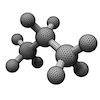
\includegraphics{images/logo.jpeg}\\
			To become the first logo for BU ProPANE.
			
		\subsection{Document Template}
			Decide to use \LaTeX as the default formatter for all formal documents. Decided on \LaTeX because it does the formatting and we want to focus on getting information on paper rather than formatting. \\
			\\
			The default template will start with a title page. The title page will include the title of the document as well as the names of the authors, the date it was created, and a summary of the contents of the document. The body of the document will be formatted using \LaTeX section, subsection, and subsubsection commands. 
			

\end{document}